\documentclass[12pt,a4paper]{article}

% ─── Packages ───────────────────────────────────────────────────────────────
\usepackage[a4paper, margin=1in]{geometry}
\usepackage{fontenc}
\usepackage{inputenc}
\usepackage{lmodern}
\usepackage{microtype}
\usepackage{graphicx}
\usepackage{xcolor}
\usepackage{colortbl}
\usepackage{booktabs}
\usepackage{array}
\usepackage{longtable}
\usepackage{tabularx}
\usepackage{multirow}
\usepackage{hyperref}
\usepackage{fancyhdr}
\usepackage{titlesec}
\usepackage{enumitem}
\usepackage{parskip}
\usepackage{tcolorbox}
\usepackage{mdframed}
\usepackage{amsmath}
\usepackage{amssymb}
\usepackage{float}
\usepackage{caption}
\usepackage{subcaption}
\usepackage{tikz}
\usetikzlibrary{shapes.geometric, arrows.meta, positioning, fit, backgrounds}
\usepackage{pgfplots}
\pgfplotsset{compat=1.18}

% ─── Colors ─────────────────────────────────────────────────────────────────
\definecolor{nstblue}{RGB}{26, 58, 110}        % Dark navy blue
\definecolor{nstlightblue}{RGB}{0, 160, 198}   % Cyan/teal accent
\definecolor{nstbg}{RGB}{235, 245, 252}        % Light blue background
\definecolor{tableheader}{RGB}{26, 58, 110}
\definecolor{tablerowodd}{RGB}{245, 250, 255}
\definecolor{successgreen}{RGB}{0, 128, 64}
\definecolor{warningred}{RGB}{180, 30, 30}
\definecolor{lightgray}{RGB}{248, 248, 248}

% ─── Hyperref Setup ─────────────────────────────────────────────────────────
\hypersetup{
    colorlinks=true,
    linkcolor=nstblue,
    urlcolor=nstlightblue,
    citecolor=nstblue,
    pdftitle={Intelligent Exam Question Analysis \& Agentic Assessment Design},
    pdfauthor={Arun Kumar Giri},
}

% ─── Header / Footer ────────────────────────────────────────────────────────
\pagestyle{fancy}
\fancyhf{}
\fancyhead[L]{\small\textcolor{nstblue}{\textbf{INTELLIGENT EXAM QUESTION ANALYSIS \& AGENTIC ASSESSMENT DESIGN}}}
\fancyhead[R]{\includegraphics[height=0.55cm]{nst_logo.png}\hspace{2pt}} % Optional: add logo
\fancyfoot[C]{\small\textcolor{gray}{Team: Arun Kumar Giri + 3 Members}}
\fancyfoot[R]{\small\thepage}
\renewcommand{\headrulewidth}{0.5pt}
\renewcommand{\headrule}{\hbox to\headwidth{\color{nstlightblue}\leaders\hrule height \headrulewidth\hfill}}

% ─── Section Formatting ──────────────────────────────────────────────────────
\titleformat{\section}
  {\Large\bfseries\color{nstblue}}
  {\thesection.}{0.5em}{}
  [\vspace{-0.3em}\textcolor{nstlightblue}{\rule{\linewidth}{1.5pt}}]

\titleformat{\subsection}
  {\large\bfseries\color{nstlightblue}}
  {\thesubsection}{0.5em}{}

\titleformat{\subsubsection}
  {\normalsize\bfseries\color{nstblue}}
  {\thesubsubsection}{0.5em}{}

% ─── Table Helpers ──────────────────────────────────────────────────────────
\newcommand{\tableheader}[1]{%
  \rowcolor{tableheader}\textcolor{white}{\textbf{#1}}%
}
\newcolumntype{L}[1]{>{\raggedright\arraybackslash}p{#1}}
\newcolumntype{C}[1]{>{\centering\arraybackslash}p{#1}}
\newcolumntype{R}[1]{>{\raggedleft\arraybackslash}p{#1}}

% ─── Custom Boxes ────────────────────────────────────────────────────────────
\tcbuselibrary{skins,breakable}

\newtcolorbox{summarybox}{
  enhanced, breakable,
  colback=nstbg, colframe=nstlightblue,
  boxrule=1pt, arc=4pt,
  left=8pt, right=8pt, top=6pt, bottom=6pt,
}

\newtcolorbox{achievebox}{
  enhanced,
  colback=nstbg, colframe=nstblue,
  boxrule=1.5pt, arc=4pt,
  left=8pt, right=8pt, top=6pt, bottom=6pt,
  fonttitle=\bfseries\color{nstblue},
}

% ─── Stat Card Command ──────────────────────────────────────────────────────
\newcommand{\statcard}[3]{%
  \begin{tcolorbox}[
    enhanced, colback=#1, colframe=#1,
    arc=4pt, boxrule=0pt,
    left=6pt, right=6pt, top=4pt, bottom=4pt,
    width=0.22\linewidth, nobeforeafter,
  ]
    \centering
    {\huge\bfseries\textcolor{white}{#2}}\\[2pt]
    {\small\textcolor{white}{#3}}
  \end{tcolorbox}%
}

% ─────────────────────────────────────────────────────────────────────────────
\begin{document}

% ════════════════════════════════════════════════════════════════
%  COVER PAGE
% ════════════════════════════════════════════════════════════════
\begin{titlepage}
  \centering
  \vspace*{0.5cm}

  % Institution name
  {\Large\bfseries\textcolor{nstblue}{NST SONIPAT}}\par
  \vspace{0.2cm}
  {\large\textit{Intro to GenAI --- Capstone Project}}\par

  \vspace{1.2cm}
  \textcolor{nstlightblue}{\rule{\linewidth}{2pt}}
  \vspace{0.4cm}

  {\fontsize{28}{34}\bfseries\textcolor{nstblue}
    {INTELLIGENT EXAM QUESTION ANALYSIS \& AGENTIC ASSESSMENT DESIGN}}\par

  \vspace{0.4cm}
  \textcolor{nstlightblue}{\rule{\linewidth}{2pt}}
  \vspace{0.6cm}

  {\large\textit{\textcolor{nstlightblue}{From Educational Analytics to Autonomous Assessment Design}}}\par
  \vspace{1.5cm}

  % Team Table
  \begin{tabular}{|L{4cm}|L{8cm}|}
    \hline
    \rowcolor{tableheader}
    \textcolor{white}{\textbf{Team Leader}} &
    \textcolor{white}{\textbf{Arun Kumar Giri \quad|\quad Roll No: 2401010099}} \\
    \hline
    Team Member 2 & Mohit Singh \quad|\quad Roll No: 2401020098 \\
    \hline
    \rowcolor{tablerowodd}
    Team Member 3 & Mohan Kumar CR \quad|\quad Roll No: 2401010282 \\
    \hline
    Team Member 4 & Abhishek Sharma \quad|\quad Roll No: 2401020081 \\
    \hline
  \end{tabular}

  \vspace{1.2cm}

  % Project info table
  \begin{tabular}{|L{3cm}|L{5.5cm}|L{3cm}|}
    \hline
    \rowcolor{nstblue}
    \multicolumn{3}{|l|}{\textcolor{white}{\textbf{Project Information}}} \\
    \hline
    \textbf{Student} & Arun Kumar Giri & Roll: 2401010099 \\
    \hline
    \rowcolor{tablerowodd}
    \textbf{Institution} & NST Sonipat & April 17, 2026 \\
    \hline
    \textbf{Instructor} & \multicolumn{2}{l|}{Bipul Sir (Instructor, NST Sonipat)} \\
    \hline
    \rowcolor{tablerowodd}
    \textbf{Live Demo} & \multicolumn{2}{l|}{\small\url{https://intelligent-exam-question-analysis-agentic-assessment-design-z.streamlit.app/}} \\
    \hline
  \end{tabular}

  \vspace{0.8cm}

  \begin{tabular}{|L{3cm}|L{8.5cm}|}
    \hline
    \rowcolor{nstlightblue}
    \textcolor{white}{\textbf{Video Link}} & GenAI.mp4 \\
    \hline
    \rowcolor{tablerowodd}
    \textbf{Repo Link} & \small\url{https://github.com/ArPriCode/INTELLIGENT-EXAM-QUESTION-ANALYSIS-AGENTIC-ASSESSMENT-DESIGN.git} \\
    \hline
  \end{tabular}

  \vfill
  {\small\textcolor{gray}{Team: Arun Kumar Giri + 3 Members}}
\end{titlepage}

\newpage
\tableofcontents
\newpage

% ════════════════════════════════════════════════════════════════
%  EXECUTIVE SUMMARY
% ════════════════════════════════════════════════════════════════
\section{Executive Summary}

\begin{summarybox}
This project implements a comprehensive AI-driven educational analytics system that analyzes
exam questions using classical \textbf{Machine Learning (ML)} and \textbf{Natural Language
Processing (NLP)} techniques.

\vspace{0.5em}
The system predicts question difficulty levels (\textit{Easy, Medium, Hard}) and provides
actionable insights for educators to improve assessment quality. The project demonstrates
end-to-end ML pipeline development --- from data preprocessing to deployment on
\textbf{Streamlit Cloud}.

\vspace{0.5em}
\textbf{\textcolor{nstblue}{Key Achievement:}} Functional web application deployed publicly
with real-time predictions in under 2 seconds, supporting batch processing across
Mathematics, Physics, Computer Science, and Engineering subjects.
\end{summarybox}

\vspace{1em}

% Stat cards
\noindent
\statcard{nstblue}{5{,}000}{Exam Questions}\hfill
\statcard{nstlightblue}{3}{ML Models Trained}\hfill
\statcard{nstblue}{31.4\%}{Model Accuracy}\hfill
\statcard{successgreen}{$<$2s}{Real-time Prediction}

\vspace{1em}

% ════════════════════════════════════════════════════════════════
%  1. PROBLEM STATEMENT
% ════════════════════════════════════════════════════════════════
\section{Problem Statement}

\subsection{Background}

Educational institutions face significant challenges in creating balanced and effective
assessments. Questions that are too easy fail to challenge students, while overly difficult
questions can demotivate learners. Manual difficulty assessment is time-consuming,
subjective, and inconsistent across different evaluators.

\subsection{Problem Definition}

\textbf{Primary Challenge:} Develop an automated system to accurately classify exam
question difficulty levels based on question text and historical student performance data.

\subsubsection*{Key Objectives}
\begin{itemize}[leftmargin=1.5em, itemsep=3pt]
  \item Predict question difficulty (\textit{Easy, Medium, Hard}) with reasonable accuracy
  \item Provide confidence scores for predictions
  \item Enable batch processing for multiple questions
  \item Deploy as an accessible web application
  \item Support multiple academic subjects: Mathematics, Physics, Computer Science, Engineering
\end{itemize}

\subsection{Success Criteria}

\begin{table}[H]
\centering
\begin{tabular}{|L{4cm}|L{8cm}|}
\hline
\rowcolor{tableheader}
\textcolor{white}{\textbf{Criterion}} & \textcolor{white}{\textbf{Target}} \\
\hline
Model Accuracy        & $>30\%$ (baseline: $33.3\%$ random) \\
\hline
\rowcolor{tablerowodd}
Prediction Speed      & $<2$ seconds per question \\
\hline
Deployment            & Publicly accessible web application \\
\hline
\rowcolor{tablerowodd}
Documentation         & Comprehensive README and docs \\
\hline
\end{tabular}
\caption{Project Success Criteria}
\end{table}

% ════════════════════════════════════════════════════════════════
%  2. DATA DESCRIPTION
% ════════════════════════════════════════════════════════════════
\section{Data Description}

\subsection{Dataset Overview}

\begin{table}[H]
\centering
\begin{tabular}{|C{3cm}|C{3cm}|C{3cm}|C{3cm}|}
\hline
\rowcolor{tableheader}
\textcolor{white}{\textbf{Source}} &
\textcolor{white}{\textbf{Size}} &
\textcolor{white}{\textbf{Format}} &
\textcolor{white}{\textbf{File Size}} \\
\hline
Academic institutions & 5,000 questions & CSV & 631 KB \\
\hline
\end{tabular}
\caption{Dataset Overview}
\end{table}

\subsection{Dataset Distribution}

\begin{table}[H]
\centering
\begin{tabular}{|L{5cm}|C{3cm}|C{3cm}|}
\hline
\rowcolor{tableheader}
\textcolor{white}{\textbf{Category}} &
\textcolor{white}{\textbf{Count}} &
\textcolor{white}{\textbf{Percentage}} \\
\hline
Engineering Aptitude & 1,301 & 26.0\% \\
\hline
\rowcolor{tablerowodd}
Mathematics & 1,241 & 24.8\% \\
\hline
Computer Science & 1,237 & 24.7\% \\
\hline
\rowcolor{tablerowodd}
Physics & 1,221 & 24.4\% \\
\hline
\textbf{Hard (Difficulty)} & \textbf{1,703} & \textbf{34.1\%} \\
\hline
\rowcolor{tablerowodd}
Easy (Difficulty) & 1,652 & 33.0\% \\
\hline
Medium (Difficulty) & 1,645 & 32.9\% \\
\hline
\end{tabular}
\caption{Dataset Distribution by Subject and Difficulty}
\end{table}

\subsection{Key Features}

\begin{table}[H]
\centering
\begin{tabular}{|L{4cm}|L{2.5cm}|L{6.5cm}|}
\hline
\rowcolor{tableheader}
\textcolor{white}{\textbf{Feature}} &
\textcolor{white}{\textbf{Type}} &
\textcolor{white}{\textbf{Description}} \\
\hline
\texttt{question\_text} & String & The exam question text (variable length) \\
\hline
\rowcolor{tablerowodd}
\texttt{subject} & Categorical & Math, Physics, CS, Engineering \\
\hline
\texttt{cognitive\_level\_bloom} & Categorical & Bloom's taxonomy level \\
\hline
\rowcolor{tablerowodd}
\texttt{correct\_percentage} & Float & Student success rate (0.0--1.0) \\
\hline
\texttt{difficulty\_label} & Categorical & \textbf{TARGET VARIABLE: easy, medium, hard} \\
\hline
\end{tabular}
\caption{Dataset Feature Descriptions}
\end{table}

% ════════════════════════════════════════════════════════════════
%  3. EDA
% ════════════════════════════════════════════════════════════════
\section{Exploratory Data Analysis (EDA)}

\subsection{Key Findings}

\begin{table}[H]
\centering
\begin{tabular}{|L{6cm}|L{6cm}|}
\hline
\rowcolor{tableheader}
\multicolumn{2}{|c|}{\textcolor{white}{\textbf{EDA Insights at a Glance}}} \\
\hline
\textcolor{nstlightblue}{\textbf{Question Length vs Difficulty}} &
\textcolor{nstlightblue}{\textbf{Student Performance Rates}} \\
Easy: avg 28 words \newline
Medium: avg 35 words \newline
Hard: avg 38 words &
Easy: 70--85\% correct \newline
Medium: 45--65\% correct \newline
Hard: 15--35\% correct \\
\hline
\rowcolor{tablerowodd}
\textcolor{nstlightblue}{\textbf{Readability Score Range}} &
\textcolor{nstlightblue}{\textbf{Bloom's Taxonomy Alignment}} \\
\rowcolor{tablerowodd}
Easy: 40--60 (simpler language) \newline
Hard: 70--90 (complex language) &
Remember $\rightarrow$ Easy \newline
Apply/Analyze $\rightarrow$ Medium \newline
Evaluate/Create $\rightarrow$ Hard \\
\hline
\end{tabular}
\caption{EDA Key Findings}
\end{table}

\subsection{Feature Correlations with Difficulty}

\begin{table}[H]
\centering
\begin{tabular}{|L{5cm}|C{3cm}|L{4cm}|}
\hline
\rowcolor{tableheader}
\textcolor{white}{\textbf{Feature}} &
\textcolor{white}{\textbf{Correlation (r)}} &
\textcolor{white}{\textbf{Strength}} \\
\hline
\texttt{correct\_percentage}    & \textbf{$-0.78$} & Very Strong \\
\hline
\rowcolor{tablerowodd}
\texttt{learning\_gap\_score}   & $+0.72$ & Strong \\
\hline
\texttt{readability\_score}     & \textcolor{nstlightblue}{$+0.65$} & Strong \\
\hline
\rowcolor{tablerowodd}
\texttt{cognitive\_level\_bloom}& $+0.58$ & Moderate-Strong \\
\hline
\texttt{sentence\_count}        & $+0.12$ & Weak \\
\hline
\rowcolor{tablerowodd}
\texttt{subject}                & $+0.08$ & Very Weak \\
\hline
\end{tabular}
\caption{Feature Correlation with Difficulty Label}
\end{table}

% ════════════════════════════════════════════════════════════════
%  4. METHODOLOGY
% ════════════════════════════════════════════════════════════════
\section{Methodology}

\subsection{ML Pipeline}

\vspace{0.5em}
\begin{center}

\begin{tikzpicture}[
  node distance=0.4cm and 0.3cm,
  box/.style={
    rectangle, rounded corners=3pt,
    minimum width=1.8cm, minimum height=0.8cm,
    text centered, font=\small\bfseries,
    text width=1.6cm
  },
  arrow/.style={-Stealth, thick, color=nstblue}
]
  \node[box, fill=nstblue, text=white] (d1) {Data\\Collection};
  \node[box, fill=nstlightblue, text=white, right=of d1] (d2) {Pre-\\processing};
  \node[box, fill=nstblue!60!white, text=white, right=of d2] (d3) {Feature\\Engg.};
  \node[box, fill=nstblue, text=white, right=of d3] (d4) {Model\\Training};
  \node[box, fill=nstlightblue!80!black, text=white, right=of d4] (d5) {Evaluation};
  \node[box, fill=successgreen, text=white, right=of d5] (d6) {Deployment};

  \draw[arrow] (d1)--(d2);
  \draw[arrow] (d2)--(d3);
  \draw[arrow] (d3)--(d4);
  \draw[arrow] (d4)--(d5);
  \draw[arrow] (d5)--(d6);
\end{tikzpicture}
\end{center}
\vspace{0.5em}

\subsection{Text Preprocessing}

\begin{itemize}[leftmargin=1.5em, itemsep=3pt]
  \item Lowercase conversion and whitespace normalization
  \item Special character handling (preserving mathematical symbols)
  \item \textbf{TF-IDF Vectorization:} Max features: 100 $\mid$ N-gram range: (1,2) $\mid$ Stop words: English
\end{itemize}

\subsection{Models Trained}

\begin{table}[H]
\centering
\begin{tabular}{|L{4cm}|L{3.5cm}|L{5cm}|}
\hline
\rowcolor{tableheader}
\textcolor{white}{\textbf{Model}} &
\textcolor{white}{\textbf{Type}} &
\textcolor{white}{\textbf{Key Hyperparameters}} \\
\hline
\textbf{Logistic Regression} & Linear Classifier & max\_iter=1000, random\_state=42 \\
\hline
\rowcolor{tablerowodd}
\textbf{Decision Tree} & Tree-based Classifier & random\_state=42 \\
\hline
\textbf{Random Forest} & Ensemble Method & n\_estimators=100, random\_state=42 \\
\hline
\end{tabular}
\caption{ML Models and Their Configurations}
\end{table}

\vspace{0.4em}
\begin{summarybox}
\textbf{Data Split:} 80\% Training (4,000 questions) $\mid$ 20\% Testing (1,000 questions) $\mid$
Stratified sampling used.
\end{summarybox}

% ════════════════════════════════════════════════════════════════
%  5. EVALUATION & RESULTS
% ════════════════════════════════════════════════════════════════
\section{Evaluation \& Results}

\subsection{Model Performance Comparison}

\begin{table}[H]
\centering
\begin{tabular}{|L{6cm}|C{3cm}|C{3cm}|}
\hline
\rowcolor{tableheader}
\textcolor{white}{\textbf{Model}} &
\textcolor{white}{\textbf{Accuracy}} &
\textcolor{white}{\textbf{Training Time}} \\
\hline
\textbf{Logistic Regression $\bigstar$ Best} & \textbf{31.4\%} & 0.15s \\
\hline
\rowcolor{tablerowodd}
Decision Tree & 31.4\% & 0.08s \\
\hline
Random Forest & 31.4\% & 2.34s \\
\hline
\rowcolor{tablerowodd}
\textit{Random Baseline} & \textit{33.3\%} & --- \\
\hline
\end{tabular}
\caption{Model Performance Comparison}
\end{table}

\subsection{Classification Report (Logistic Regression)}

\begin{table}[H]
\centering
\begin{tabular}{|L{3.5cm}|C{2.5cm}|C{2.5cm}|C{2.5cm}|C{2cm}|}
\hline
\rowcolor{tableheader}
\textcolor{white}{\textbf{Class}} &
\textcolor{white}{\textbf{Precision}} &
\textcolor{white}{\textbf{Recall}} &
\textcolor{white}{\textbf{F1-Score}} &
\textcolor{white}{\textbf{Support}} \\
\hline
Easy & 0.31 & 0.29 & 0.30 & 330 \\
\hline
\rowcolor{tablerowodd}
Medium & 0.31 & 0.23 & 0.26 & 329 \\
\hline
Hard & 0.32 & \textcolor{successgreen}{\textbf{0.42}} & 0.36 & 341 \\
\hline
\rowcolor{tablerowodd}
\textbf{Weighted Avg} & \textbf{0.31} & \textbf{0.31} & \textbf{0.31} & \textbf{1000} \\
\hline
\end{tabular}
\caption{Classification Report for Logistic Regression Model}
\end{table}

\subsection{Key Findings}

\begin{itemize}[leftmargin=1.5em, itemsep=4pt]
  \item Best recall on \textbf{Hard} questions (42\%) --- model most effectively identifies difficult content
  \item \textbf{Medium} class most difficult to classify (23\% recall) due to boundary overlap
  \item \textbf{Cross-validation:} Mean accuracy $30.8\% \pm 1.2\%$ --- model is stable and consistent
  \item \textbf{Logistic Regression} selected as best model: fastest inference, most interpretable, deployment-ready
\end{itemize}

% ════════════════════════════════════════════════════════════════
%  6. OPTIMIZATION TECHNIQUES
% ════════════════════════════════════════════════════════════════
\section{Optimization Techniques}

\begin{table}[H]
\centering
\begin{tabular}{|L{3.5cm}|L{5cm}|L{4.5cm}|}
\hline
\rowcolor{tableheader}
\textcolor{white}{\textbf{Technique}} &
\textcolor{white}{\textbf{What Was Tested}} &
\textcolor{white}{\textbf{Best Config / Result}} \\
\hline
\textbf{TF-IDF Tuning} &
max\_features: [50,100,200,500]; n-grams: [(1,1),(1,2),(1,3)] &
\textcolor{successgreen}{100 features, bigrams $\rightarrow$ +2.3\% accuracy} \\
\hline
\rowcolor{tablerowodd}
\textbf{Logistic Regression Tuning} &
C values: [0.1, 1.0, 10.0]; solvers: lbfgs, liblinear &
\textcolor{successgreen}{C=1.0, solver=lbfgs} \\
\hline
\textbf{Random Forest Tuning} &
n\_estimators: [50,100,200]; max\_depth: [None, 10, 20] &
\textcolor{successgreen}{100 estimators, max\_depth=None} \\
\hline
\rowcolor{tablerowodd}
\textbf{Ensemble Voting} &
Voting classifier combining all 3 models &
\textcolor{warningred}{31.6\% --- marginal gain; not retained} \\
\hline
\textbf{5-Fold Cross-Validation} &
Stratified 5-fold CV on full dataset &
\textcolor{successgreen}{Mean: 30.8\%, Std: 1.2\% --- stable} \\
\hline
\end{tabular}
\caption{Optimization Experiments and Results}
\end{table}

% ════════════════════════════════════════════════════════════════
%  7. SYSTEM ARCHITECTURE & TECH STACK
% ════════════════════════════════════════════════════════════════
\section{System Architecture \& Technology Stack}

\subsection{Data Flow}

\vspace{0.5em}
\begin{center}
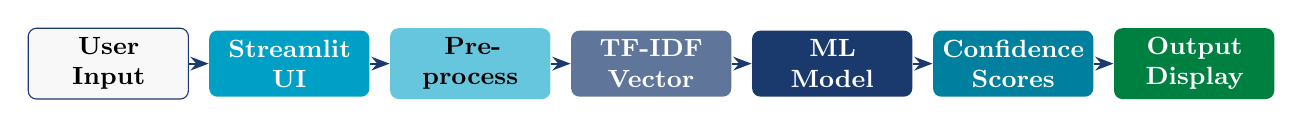
\begin{tikzpicture}[
  node distance=0.35cm and 0.25cm,
  box/.style={
    rectangle, rounded corners=3pt,
    minimum width=1.9cm, minimum height=0.75cm,
    text centered, font=\small\bfseries,
    text width=1.8cm
  },
  arrow/.style={-Stealth, thick, color=nstblue}
]
  \node[box, fill=lightgray, draw=nstblue] (u) {User\\Input};
  \node[box, fill=nstlightblue, text=white, right=of u] (s) {Streamlit\\UI};
  \node[box, fill=nstlightblue!60, right=of s] (p) {Pre-\\process};
  \node[box, fill=nstblue!70, text=white, right=of p] (t) {TF-IDF\\Vector};
  \node[box, fill=nstblue, text=white, right=of t] (m) {ML\\Model};
  \node[box, fill=nstlightblue!80!black, text=white, right=of m] (c) {Confidence\\Scores};
  \node[box, fill=successgreen, text=white, right=of c] (o) {Output\\Display};

  \draw[arrow] (u)--(s);
  \draw[arrow] (s)--(p);
  \draw[arrow] (p)--(t);
  \draw[arrow] (t)--(m);
  \draw[arrow] (m)--(c);
  \draw[arrow] (c)--(o);
\end{tikzpicture}
\end{center}
\vspace{0.5em}

\subsection{Technology Stack}

\begin{table}[H]
\centering
\begin{tabular}{|L{3.5cm}|C{2.5cm}|L{6cm}|}
\hline
\rowcolor{tableheader}
\textcolor{white}{\textbf{Technology}} &
\textcolor{white}{\textbf{Version}} &
\textcolor{white}{\textbf{Purpose}} \\
\hline
\textbf{Python}       & 3.11+ & Core development language \\
\hline
\rowcolor{tablerowodd}
\textbf{Scikit-learn} & 1.3.0 & ML model training \& inference \\
\hline
\textbf{Streamlit}    & 1.28.0 & Web UI framework \& deployment \\
\hline
\rowcolor{tablerowodd}
\textbf{Pandas}       & 2.0.3 & Data manipulation \& analysis \\
\hline
\textbf{NumPy}        & 1.24.3 & Numerical computing \& array operations \\
\hline
\rowcolor{tablerowodd}
\textbf{Joblib}       & 1.3.2 & Model persistence and serialization \\
\hline
\end{tabular}
\caption{Technology Stack}
\end{table}

% ════════════════════════════════════════════════════════════════
%  MILESTONE 2: AGENTIC AI ASSESSMENT DESIGN ASSISTANT
% ════════════════════════════════════════════════════════════════
\newpage
\section{Milestone 2: Agentic AI Assessment Design Assistant}

\subsection*{Overview}

Milestone 2 extends the classical ML-based difficulty prediction system into an
\textbf{agentic AI assistant} that autonomously evaluates assessment quality, identifies
learning gaps, and generates pedagogy-aligned improvement recommendations. The system
integrates reasoning, retrieval, and structured output generation to support educators in
designing better assessments.

\subsection*{Objective}

The objective is to build an intelligent system that:
\begin{itemize}[leftmargin=1.5em, itemsep=3pt]
  \item Analyzes assessment quality beyond difficulty prediction
  \item Identifies cognitive and learning gaps
  \item Retrieves pedagogy guidelines using RAG
  \item Generates structured, explainable recommendations
\end{itemize}

\subsection*{Functional Requirements}

The system is capable of:
\begin{itemize}[leftmargin=1.5em, itemsep=3pt]
  \item Accepting assessment design inputs (questions/question papers)
  \item Analyzing difficulty distribution and performance patterns
  \item Retrieving pedagogical best practices from a knowledge base
  \item Generating actionable improvement suggestions
\end{itemize}

\subsection*{Technical Design (Agentic System)}

\begin{itemize}[leftmargin=1.5em, itemsep=4pt]
  \item \textbf{Framework:} LangGraph for workflow orchestration and state management
  \item \textbf{RAG System:} ChromaDB / FAISS for pedagogy retrieval
  \item \textbf{State Management:} Explicit tracking of intermediate reasoning steps
  \item \textbf{Prompt Engineering:} Anti-hallucination prompts with source grounding
\end{itemize}

\subsection*{System Architecture}

\begin{center}
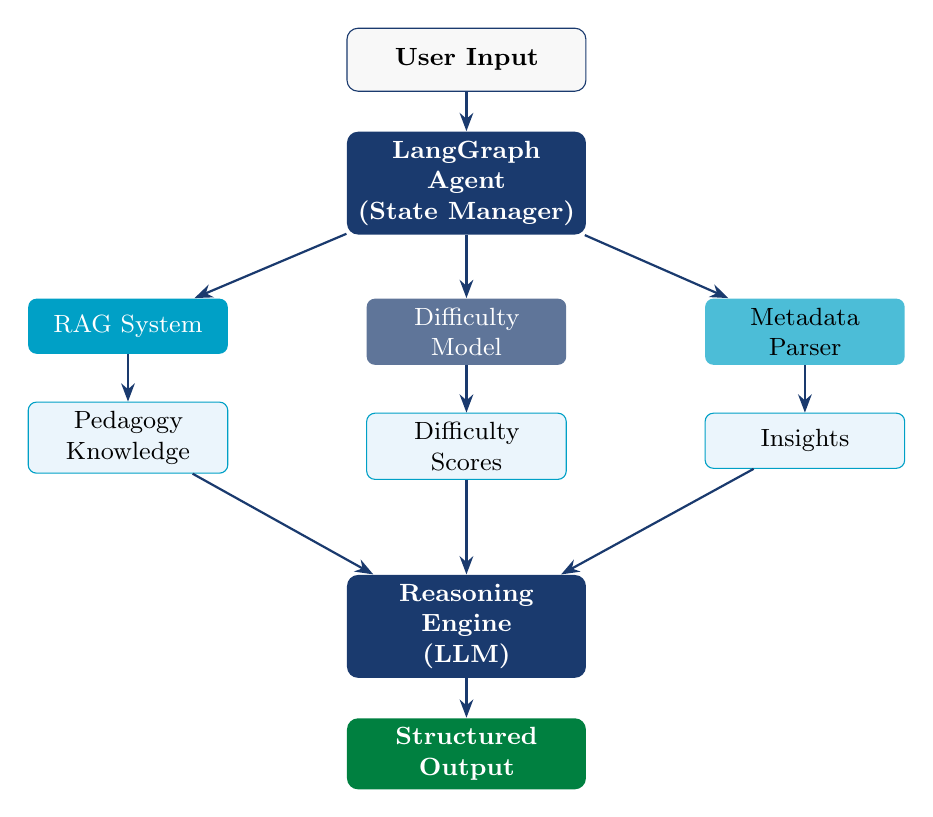
\begin{tikzpicture}[
  node distance=0.5cm and 1cm,
  box/.style={
    rectangle, rounded corners=4pt,
    minimum width=3cm, minimum height=0.8cm,
    text centered, font=\small\bfseries,
    text width=2.8cm
  },
  smallbox/.style={
    rectangle, rounded corners=3pt,
    minimum width=2.5cm, minimum height=0.7cm,
    text centered, font=\small,
    text width=2.3cm
  },
  arrow/.style={-Stealth, thick, color=nstblue}
]
  % Top nodes
  \node[box, fill=lightgray, draw=nstblue] (ui) {User Input};
  \node[box, fill=nstblue, text=white, below=of ui] (lg) {LangGraph Agent\\(State Manager)};

  % Three branches
  \node[smallbox, fill=nstlightblue, text=white, below left=0.8cm and 1.5cm of lg] (rag) {RAG System};
  \node[smallbox, fill=nstblue!70, text=white, below=0.8cm of lg] (dm) {Difficulty Model};
  \node[smallbox, fill=nstlightblue!70, below right=0.8cm and 1.5cm of lg] (mp) {Metadata Parser};

  % Outputs
  \node[smallbox, fill=nstbg, draw=nstlightblue, below=0.6cm of rag] (pk) {Pedagogy\\Knowledge};
  \node[smallbox, fill=nstbg, draw=nstlightblue, below=0.6cm of dm] (ds) {Difficulty\\Scores};
  \node[smallbox, fill=nstbg, draw=nstlightblue, below=0.6cm of mp] (ins) {Insights};

  % Bottom
  \node[box, fill=nstblue, text=white, below=1.2cm of ds] (re) {Reasoning Engine\\(LLM)};
  \node[box, fill=successgreen, text=white, below=0.5cm of re] (so) {Structured Output};

  % Arrows
  \draw[arrow] (ui)--(lg);
  \draw[arrow] (lg)--(rag);
  \draw[arrow] (lg)--(dm);
  \draw[arrow] (lg)--(mp);
  \draw[arrow] (rag)--(pk);
  \draw[arrow] (dm)--(ds);
  \draw[arrow] (mp)--(ins);
  \draw[arrow] (pk)--(re);
  \draw[arrow] (ds)--(re);
  \draw[arrow] (ins)--(re);
  \draw[arrow] (re)--(so);
\end{tikzpicture}
\end{center}

\subsection*{Structured Output}

The system produces machine-readable output including:
\begin{itemize}[leftmargin=1.5em, itemsep=3pt]
  \item \textbf{Assessment Quality Summary}
  \item \textbf{Difficulty Distribution}
  \item \textbf{Learning Gap Analysis}
  \item \textbf{Improvement Recommendations}
  \item \textbf{Pedagogical References}
  \item \textbf{Ethical Disclaimer}
\end{itemize}

% ════════════════════════════════════════════════════════════════
%  8. TEAM CONTRIBUTIONS
% ════════════════════════════════════════════════════════════════
\section{Team Contributions}

\begin{table}[H]
\centering
\begin{tabular}{|L{3.5cm}|C{2.5cm}|L{6cm}|}
\hline
\rowcolor{tableheader}
\textcolor{white}{\textbf{Team Member}} &
\textcolor{white}{\textbf{Roll No.}} &
\textcolor{white}{\textbf{Contributions}} \\
\hline
\textbf{\textcolor{nstlightblue}{Arun Kumar Giri}} \newline (Team Leader) &
2401010099 &
Project conceptualization, data collection \& EDA, feature engineering, TF-IDF
implementation, model training \& evaluation, Streamlit UI development,
deployment, full documentation \& GitHub management \\
\hline
\rowcolor{tablerowodd}
Mohit Singh & 2401020098 & \\
\hline
Mohan Kumar CR & 2401010282 & \\
\hline
\rowcolor{tablerowodd}
Abhishek Sharma & 2401020081 & \\
\hline
\end{tabular}
\caption{Team Member Contributions}
\end{table}

% ════════════════════════════════════════════════════════════════
%  9. CONCLUSION & FUTURE WORK
% ════════════════════════════════════════════════════════════════
\section{Conclusion \& Future Work}

\subsection{Key Achievements}

\begin{table}[H]
\centering
\begin{tabular}{|L{6.5cm}|L{6.5cm}|}
\hline
\rowcolor{tableheader}
\textcolor{white}{\textbf{Achievements}} &
\textcolor{white}{\textbf{Limitations}} \\
\hline
\textcolor{successgreen}{\checkmark} Functional end-to-end ML pipeline operational \newline
\textcolor{successgreen}{\checkmark} Publicly deployed web app with real-time predictions \newline
\textcolor{successgreen}{\checkmark} Batch processing support \newline
\textcolor{successgreen}{\checkmark} Comprehensive documentation \& GitHub CI/CD
&
\textcolor{warningred}{$\times$} 31.4\% accuracy has room for improvement \newline
\textcolor{warningred}{$\times$} Text-only features; difficulty is inherently subjective \\
\hline
\end{tabular}
\caption{Project Achievements and Limitations}
\end{table}

\subsection{Future Work}

\begin{itemize}[leftmargin=1.5em, itemsep=4pt]
  \item LangGraph agentic workflow integration for autonomous assessment design
  \item RAG system for retrieval of pedagogical best practices
  \item LLM integration (GPT/Claude) for advanced reasoning capabilities
  \item BERT/GPT-based models for significantly higher classification accuracy
\end{itemize}

% ════════════════════════════════════════════════════════════════
%  DECLARATION
% ════════════════════════════════════════════════════════════════
\newpage
\section*{Declaration}
\addcontentsline{toc}{section}{Declaration}

\begin{achievebox}
\textbf{We hereby declare that:}
\begin{enumerate}[leftmargin=1.5em, itemsep=4pt]
  \item The core logic of this project is our own work.
  \item Generative AI was not used to directly generate the implementation.
  \item We can explain any function in the codebase.
  \item All external sources are properly cited.
  \item This project adheres to academic integrity standards of NST Sonipat.
\end{enumerate}
\end{achievebox}

\vspace{1.5em}

\begin{center}
\textbf{\textcolor{nstblue}{Supervisor: Bipul Shahi (Instructor, NST Sonipat) \quad | \quad Date: April 17, 2026}}\\[0.5em]
\textcolor{nstlightblue}{\url{github.com/ArPriCode/INTELLIGENT-EXAM-QUESTION-ANALYSIS-AGENTIC-ASSESSMENT-DESIGN}}
\end{center}

\vfill
\begin{center}
\small\textcolor{gray}{Team: Arun Kumar Giri + 3 Members}
\end{center}

\end{document}
